\documentclass[preprint,12pt,aps,pra,showkeys,amsmath,amssymb,superscriptaddress,floatfix]{revtex4-2}
\usepackage[T1]{fontenc}
\usepackage[utf8]{inputenc}
\usepackage{amsmath,amssymb,amsthm,mathtools,mathrsfs}
\usepackage{microtype,booktabs,enumitem}
\usepackage{xcolor,tikz,etoolbox}
\usepackage[skins,breakable]{tcolorbox}
\usepackage{needspace}
% Keep diagram geometry independent of REVTeX preprint body spacing.
\AtBeginEnvironment{tikzpicture}{\linespread{1}\selectfont}
\usetikzlibrary{arrows.meta,positioning,calc,fit,decorations.pathreplacing}
\usepackage{graphicx}
\usepackage{hyperref}

\definecolor{MMBlue}{RGB}{0,82,155}
\definecolor{MMOrange}{RGB}{200,80,0}
\tikzset{
 mmnode/.style={draw=MMBlue,rounded corners=2pt,fill=MMBlue!4,align=left,execute at begin node={\raggedright},text width=5cm,font=\fontsize{10}{12}\selectfont,inner sep=6pt},
 mmimport/.style={mmnode,draw=black!65,fill=black!4},
 mmcandidate/.style={mmnode,draw=MMOrange,dashed,fill=MMOrange!5},
 mmrejected/.style={mmnode,draw=black,densely dotted,fill=black!8},
 mmproof/.style={->,thick,MMBlue},
 mmflow/.style={->,semithick,black!70},
 mmrepair/.style={->,dashed,thick,MMOrange},
 mmcandidatearrow/.style={->,dashed,semithick,MMOrange},
 mmnote/.style={font=\scriptsize,fill=white,inner sep=2pt,align=center}}

\usepackage[section]{placeins}
\setlength{\emergencystretch}{3em}
\setlist{itemsep=3pt,topsep=4pt}
\newtheorem{theorem}{Theorem}[section]
\newtheorem{proposition}[theorem]{Proposition}
\newtheorem{lemma}[theorem]{Lemma}
\newtheorem{corollary}[theorem]{Corollary}
\theoremstyle{definition}
\newtheorem{definition}[theorem]{Definition}
\newtheorem{example}[theorem]{Example}
\theoremstyle{remark}
\newtheorem{remark}[theorem]{Remark}
% Avoid isolated statement headings and single-line paragraph fragments.
\BeforeBeginEnvironment{theorem}{\Needspace{6\baselineskip}}
\BeforeBeginEnvironment{definition}{\Needspace{5\baselineskip}}
\BeforeBeginEnvironment{proposition}{\Needspace{5\baselineskip}}
\BeforeBeginEnvironment{lemma}{\Needspace{5\baselineskip}}
\BeforeBeginEnvironment{corollary}{\Needspace{5\baselineskip}}
\clubpenalty=5000
\widowpenalty=5000
\newcommand{\R}{\mathbb R}\newcommand{\Z}{\mathbb Z}\newcommand{\N}{\mathbb N}
\newcommand{\Pa}{\operatorname{Pa}}\newcommand{\Desc}{\operatorname{Desc}}
\newcommand{\cl}{\operatorname{cl}}\newcommand{\cost}{\operatorname{cost}}
\newcommand{\status}{\operatorname{status}}
% Faculty cards: a visual rail groups the five faculties within one agent.
% The rail has no arrowhead and does not represent a proof dependency.
\newcommand{\mmfacultybadge}[1]{%
 \node[circle,draw=MMBlue,line width=1pt,fill=white,
 minimum size=7mm,inner sep=0pt,font=\sffamily\small\bfseries,text=MMBlue]
 at ([xshift=15pt,yshift=-15pt]frame.north west) {#1};}
\newcommand{\mmfacultyrail}{%
 \draw[MMBlue!80,line width=1pt]
 ([xshift=15pt,yshift=2pt]frame.north west)--
 ([xshift=15pt,yshift=-2pt]frame.south west);}
\newtcolorbox{mmfacultybox}[2]{enhanced,breakable,
 colback=MMBlue!4,colframe=MMBlue!4,boxrule=0pt,arc=3pt,
 left=39pt,right=9pt,top=4pt,bottom=4pt,
 before skip=2pt,after skip=2pt,
 fontupper=\small\linespread{1.1}\selectfont,
 overlay unbroken={\mmfacultyrail\mmfacultybadge{#1}},
 overlay first={\mmfacultyrail\mmfacultybadge{#1}},
 overlay middle={\mmfacultyrail},overlay last={\mmfacultyrail}}
\newcommand{\mmfaculty}[3]{%
 \begin{mmfacultybox}{#1}{#2}
 {\sffamily\bfseries\color{MMBlue}#2}\par\smallskip #3
 \end{mmfacultybox}}
\newcommand{\agent}[9]{%
 \Needspace{8\baselineskip}
 \subsubsection{#1}
 \noindent\textbf{Object.} #2\par
 \noindent\textbf{Role.} #3\par\smallskip
 \mmfaculty{E}{Ego}{#4}
 \mmfaculty{M}{Memory}{#5}
 \mmfaculty{I}{Intellect}{#6}
 \mmfaculty{S}{Sense}{#7}
 \mmfaculty{A}{Action}{#8}
 \smallskip\noindent #9\par}

\usepackage{longtable,array,calc}
\providecommand{\tightlist}{\setlength{\itemsep}{2pt}\setlength{\parskip}{0pt}}
\makeatletter
\def\frontmatter@abstract@produce{\par\addvspace{\frontmatter@preabstractspace}%
\begingroup\prep@absbox\unvbox\absbox\post@absbox\endgroup
\addvspace{\frontmatter@postabstractspace}}
\makeatother
\newcommand{\field}[2]{\par\smallskip\noindent\textbf{#1.} #2\par}
\setlength{\emergencystretch}{5em}
\AtBeginEnvironment{verbatim}{\small\linespread{1.0}\selectfont}


\hypersetup{colorlinks=true,linkcolor=MMBlue,urlcolor=MMBlue,pdfauthor={Dibakar Sigdel}}

\begin{document}

\title{Gauss' Theorema Egregium\\[4pt]\large An End-to-End Meta-Math Walkthrough}

\author{Dibakar Sigdel}

\affiliation{Mindverse Computing LLC, Lynnwood, WA 98087, USA}

\date{October 2026}

\begin{abstract}

A complete authored walkthrough of gauss' theorema egregium, with
explicit mathematical contracts, local verification gates, and reusable
exports. The report presents the target theorem, declared imports, a
dependency graph, five-faculty node contracts, a continuous proof, a
worked example, and a hypothesis-repair audit. It is an authored
mathematical exposition, not a deployed-agent transcript or a formal
proof-assistant certificate.

\end{abstract}\maketitle\linespread{1.12}\selectfont

\noindent\textbf{DG-03 / Differential Geometry / Report v1}

\section{Target and import contract}

\begin{theorem}

For a smooth regular surface in \(\mathbb R^3\), prove Gaussian
curvature \(K=\det S\) is determined by the first fundamental form and
is preserved by local isometries.

\end{theorem}

\subsection{Foundations and permitted imports}

For a regular surface choose local coordinates and a unit normal
\(\nu\). Use the induced metric g, its Levi-Civita connection
\(\nabla\), and decomposition of the ambient derivative
\(D_XY=\nabla _XY+h(X,Y)\nu\) with \(D_X\nu =-SX\) and
\(h(X,Y)=g(SX,Y)\). These follow from orthogonal projection, metric
compatibility, and torsion-freeness. Curvature convention
\(R(X,Y)Z=\nabla _X\nabla _YZ-\nabla _Y\nabla _XZ-\nabla _[X,Y]Z\). The
Gauss equation is derived here.

\clearpage\section{Node interaction workflow}

\begin{center}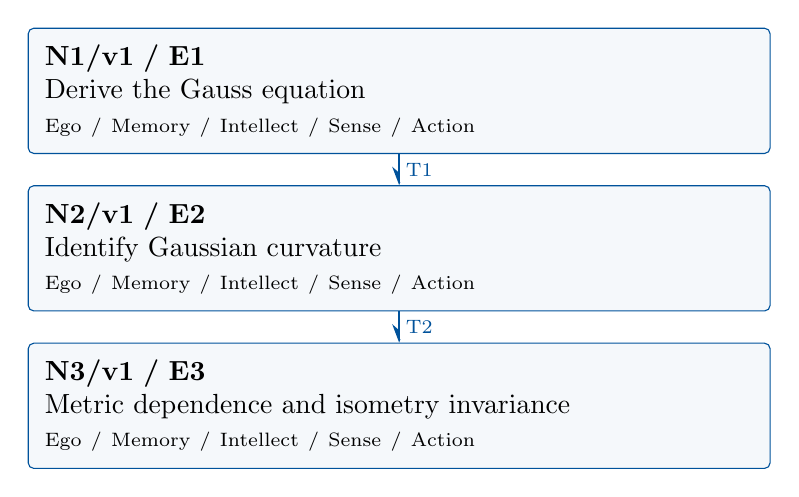
\begin{tikzpicture}[>=Stealth,x=1cm,y=1cm]

\node[mmnode,text width=9cm,minimum height=1.25cm] (N1) at (0,0.0) {\textbf{N1/v1 / E1}\\Derive the Gauss equation\\{\scriptsize Ego / Memory / Intellect / Sense / Action}};

\node[mmnode,text width=9cm,minimum height=1.25cm] (N2) at (0,-2.0) {\textbf{N2/v1 / E2}\\Identify Gaussian curvature\\{\scriptsize Ego / Memory / Intellect / Sense / Action}};

\node[mmnode,text width=9cm,minimum height=1.25cm] (N3) at (0,-4.0) {\textbf{N3/v1 / E3}\\Metric dependence and isometry invariance\\{\scriptsize Ego / Memory / Intellect / Sense / Action}};

\draw[mmproof] (N1.south) -- node[mmnote,right] {T1} (N2.north);

\draw[mmproof] (N2.south) -- node[mmnote,right] {T2} (N3.north);

\end{tikzpicture}\end{center}

Each box is one mathematical agent containing all five faculties. Blue
arrows carry the versioned exports listed below. The layout gives a
reading order; only drawn arrows assert dependencies. Diagnostic repair
is separate from the proof DAG.

\subsection{Versioned evidence-transfer ledger}

\begingroup\small\linespread{1.05}\selectfont

\Needspace{5\baselineskip}\field{T1: N1/E1/v1 to N2}{Intrinsic curvature expressed through h with its exact signs.}

\field{Receiving activity}{N2: Identify Gaussian curvature}

\field{Compatibility}{Use the same mathematical objects and hypotheses as the source export.
Receiving contract: Orthonormal tangent basis \(e_{1},e_{2}\); prior
exports E1/v1}

\Needspace{5\baselineskip}\field{T2: N2/E2/v1 to N3}{\(K=\operatorname{det} S\) is the scalar computed from the intrinsic
curvature tensor.}

\field{Receiving activity}{N3: Metric dependence and isometry invariance}

\field{Compatibility}{Use the same mathematical objects and hypotheses as the source export.
Receiving contract: Coordinate curvature formula and metric
compatibility; prior exports E2/v1}

\endgroup

\clearpage\section{Agent roles and five-faculty activities}\begingroup\small\linespread{1.05}\selectfont\setlist{itemsep=1pt,topsep=2pt}

\subsection{N1/v1: Derive the Gauss equation}

\field{Object and role}{Extract tangential terms from ambient curvature zero.}

\field{Inputs}{Flat ambient connection and tangential/normal decomposition;
foundational imports stated in §1}

\mmfaculty{E}{Ego}{Own E1/v1: Intrinsic curvature expressed through h with its exact signs.}

\mmfaculty{M}{Memory}{Retain Flat ambient connection and tangential/normal decomposition;
foundational imports stated in §1; keep their assumptions and versions
attached.}

\mmfaculty{I}{Intellect}{Extract tangential terms from ambient curvature zero.}

\mmfaculty{S}{Sense}{Changing the curvature convention changes formula signs.}

\mmfaculty{A}{Action}{Carry out the numbered deductions and publish E1/v1 together with its
hypotheses and proof location.}

\smallskip\noindent\textbf{Numbered mathematical activities}

\begin{enumerate}[label=N1.\arabic*,leftmargin=3.4em]

\item In \(R^{3}\), \(D_XD_YZ-D_YD_XZ-D_{[X,Y]}Z\)\(=0\).

\item The tangential part of \(D_XD_YZ\)
is\(\nabla_X\nabla_Y Z\)\(-h(Y,Z)SX\); interchange X,Y and subtract.

\item Therefore \(R(X,Y)Z=h(Y,Z)SX-h(X,Z)SY\).

\item Pairing with W gives \(g(R(X,Y)Z,W)=h(Y,Z)h(X,W)-h(X,Z)h(Y,W)\).

\item This is the Gauss equation with the fixed curvature convention.

\end{enumerate}

\field{Export E1/v1}{Intrinsic curvature expressed through h with its exact signs.}

\field{Acceptance gate}{Changing the curvature convention changes formula signs. Publish only
after checking every displayed deduction.}

\field{Targeted repair}{If the check fails, revise N1: Changing the curvature convention changes
formula signs. Recheck dependent nodes N2, N3.}

\clearpage

\subsection{N2/v1: Identify Gaussian curvature}

\field{Object and role}{Compute sectional curvature as a two-by-two determinant.}

\field{Inputs}{Orthonormal tangent basis \(e_{1},e_{2}\); prior exports E1/v1}

\mmfaculty{E}{Ego}{Own E2/v1: \(K=\operatorname{det} S\) is the scalar computed from the
intrinsic curvature tensor.}

\mmfaculty{M}{Memory}{Retain Orthonormal tangent basis \(e_{1},e_{2}\); prior exports E1/v1;
keep their assumptions and versions attached.}

\mmfaculty{I}{Intellect}{Compute sectional curvature as a two-by-two determinant.}

\mmfaculty{S}{Sense}{Reversing \(\nu\) negates S but preserves its two-dimensional
determinant.}

\mmfaculty{A}{Action}{Carry out the numbered deductions and publish E2/v1 together with its
hypotheses and proof location.}

\smallskip\noindent\textbf{Numbered mathematical activities}

\begin{enumerate}[label=N2.\arabic*,leftmargin=3.4em]

\item Use \(X=e_{1},Y=e_{2},Z=e_{2},W=e_{1}\).

\item The equation gives
\(g(R(e_{1},e_{2})e_{2},e_{1})=h_{11}h_{22}-h_{12}^{2}=\operatorname{det} S\),
since h is symmetric and the basis orthonormal.

\item For coordinate vectors,
\(K=g(R(\partial _{1},\partial _{2})\partial _{2},\partial _{1})/(g_{11}g_{22}-g_{12}^{2})\).

\item The denominator is positive by regularity.

\item Hence Gaussian curvature equals the intrinsic sectional curvature.

\end{enumerate}

\field{Export E2/v1}{\(K=\operatorname{det} S\) is the scalar computed from the intrinsic
curvature tensor.}

\field{Acceptance gate}{Reversing \(\nu\) negates S but preserves its two-dimensional
determinant. Publish only after checking every displayed deduction.}

\field{Targeted repair}{If the check fails, revise N2: Reversing \(\nu\) negates S but preserves
its two-dimensional determinant. Recheck dependent nodes N3.}

\clearpage

\subsection{N3/v1: Metric dependence and isometry invariance}

\field{Object and role}{Express the connection and curvature entirely through g.}

\field{Inputs}{Coordinate curvature formula and metric compatibility; prior exports
E2/v1}

\mmfaculty{E}{Ego}{Own E3/v1: Gaussian curvature is determined by the first fundamental
form and preserved by local isometries.}

\mmfaculty{M}{Memory}{Retain Coordinate curvature formula and metric compatibility; prior
exports E2/v1; keep their assumptions and versions attached.}

\mmfaculty{I}{Intellect}{Express the connection and curvature entirely through g.}

\mmfaculty{S}{Sense}{Equal extrinsic pictures are unnecessary; the connection is
metric-determined.}

\mmfaculty{A}{Action}{Carry out the numbered deductions and publish E3/v1 together with its
hypotheses and proof location.}

\smallskip\noindent\textbf{Numbered mathematical activities}

\begin{enumerate}[label=N3.\arabic*,leftmargin=3.4em]

\item The Christoffel symbols are
\(\Gamma^k_{ij}=\tfrac12 g^{k\ell}(\partial_i g_{j\ell}+\partial_j g_{i\ell}-\partial_\ell g_{ij})\).

\item In a coordinate frame \(R(\partial _i,\partial _j)\partial _k\) has
component
\(\partial_i\Gamma^\ell_{jk}-\partial_j\Gamma^\ell_{ik}+\Gamma^m_{jk}\Gamma^\ell_{im}-\Gamma^m_{ik}\Gamma^\ell_{jm}\).

\item Thus the displayed K uses only g and its first and second derivatives.

\item A local isometry preserves g and, by uniqueness of the Levi-Civita
connection, transports \(\nabla\) and R; the scalar K is consequently
preserved.

\item This proves the theorem.

\end{enumerate}

\field{Export E3/v1}{Gaussian curvature is determined by the first fundamental form and
preserved by local isometries.}

\field{Acceptance gate}{Equal extrinsic pictures are unnecessary; the connection is
metric-determined. Publish only after checking every displayed
deduction.}

\field{Targeted repair}{If the check fails, revise N3: Equal extrinsic pictures are unnecessary;
the connection is metric-determined. Withhold this terminal result until
its gate passes.}

\endgroup\clearpage\section{Continuous mathematical proof}\label{sec:proof}

Read these steps in order as one proof; the diagram is optional.
Numbered activities identify the specific constructions and deductions
owned by each node.

\subsection{§4.N1 --- Derive the Gauss
equation}\label{n1-derive-the-gauss-equation}

\begin{enumerate}
\def\labelenumi{\arabic{enumi}.}
\item
  In \(R^{3}\), \(D_XD_YZ-D_YD_XZ-D_{[X,Y]}Z\)\(=0\).
\item
  The tangential part of \(D_XD_YZ\)
  is\(\nabla_X\nabla_Y Z\)\(-h(Y,Z)SX\); interchange X,Y and subtract.
\item
  Therefore \(R(X,Y)Z=h(Y,Z)SX-h(X,Z)SY\).
\item
  Pairing with W gives \(g(R(X,Y)Z,W)=h(Y,Z)h(X,W)-h(X,Z)h(Y,W)\).
\item
  This is the Gauss equation with the fixed curvature convention.
\end{enumerate}

\subsection{§4.N2 --- Identify Gaussian
curvature}\label{n2-identify-gaussian-curvature}

\begin{enumerate}
\def\labelenumi{\arabic{enumi}.}
\item
  Use \(X=e_{1},Y=e_{2},Z=e_{2},W=e_{1}\).
\item
  The equation gives
  \(g(R(e_{1},e_{2})e_{2},e_{1})=h_{11}h_{22}-h_{12}^{2}=\operatorname{det} S\),
  since h is symmetric and the basis orthonormal.
\item
  For coordinate vectors,
  \(K=g(R(\partial _{1},\partial _{2})\partial _{2},\partial _{1})/(g_{11}g_{22}-g_{12}^{2})\).
\item
  The denominator is positive by regularity.
\item
  Hence Gaussian curvature equals the intrinsic sectional curvature.
\end{enumerate}

\subsection{§4.N3 --- Metric dependence and isometry
invariance}\label{n3-metric-dependence-and-isometry-invariance}

\begin{enumerate}
\def\labelenumi{\arabic{enumi}.}
\item
  The Christoffel symbols are
  \(\Gamma^k_{ij}=\tfrac12 g^{k\ell}(\partial_i g_{j\ell}+\partial_j g_{i\ell}-\partial_\ell g_{ij})\).
\item
  In a coordinate frame \(R(\partial _i,\partial _j)\partial _k\) has
  component
  \(\partial_i\Gamma^\ell_{jk}-\partial_j\Gamma^\ell_{ik}+\Gamma^m_{jk}\Gamma^\ell_{im}-\Gamma^m_{ik}\Gamma^\ell_{jm}\).
\item
  Thus the displayed K uses only g and its first and second derivatives.
\item
  A local isometry preserves g and, by uniqueness of the Levi-Civita
  connection, transports \(\nabla\) and R; the scalar K is consequently
  preserved.
\item
  This proves the theorem.
\end{enumerate}

\hfill$\square$

\section{Worked orchestration}

A cylinder of radiusr is parametrized by (r cosu,r sinu,v) and has
metric \(r^{2}du^{2}+dv^{2}\). Set \(x=ru,y=v\); the metric becomes
\(dx^{2}+dy^{2}\), so all \(\Gamma\) and R vanish and \(K=0\). Its
principal curvatures have one zero value, giving the same detS despite
its visible bending.

\subsection{Boundary and hypothesis audit}

A sphere has positive K whereas the plane has \(K=0\), so no local
isometry can flatten a sphere into the plane. Sense rejects equating
arbitrary bending with an isometry; the metric, not only the embedding,
must be preserved.

\section{Illustrative failure and repair}

The following is an authored diagnostic scenario. Changed assumptions
define a new contract; they do not retroactively prove the original
statement.

\subsection{Failure and correction}
This is an authored teaching trace, not a recorded agent run.

\begin{enumerate}
\def\labelenumi{\arabic{enumi}.}
\tightlist
\item
  \textbf{Ego \(\to\) Memory:} register the §1 theorem, imports, and
  requested exports before beginning the proof.
\item
  \textbf{Intellect \(\to\) Action:} choose the bridges in §3 and carry
  out the numbered activities in §4; transmit only established E-exports
  along the §2 DAG.
\item
  \textbf{Sense \(\to\) responsible node:} test the specific
  boundary/failure in §5 and the node's individual audit. A failing
  candidate is withheld; downstream nodes may not use it.
\item
  \textbf{Memory + Intellect:} identify whether the error is an omitted
  condition, an invalid inference, or an attempted extension beyond the
  theorem. Restore the exact contract or explicitly state a different
  one.
\item
  \textbf{Action:} redo the affected mathematical activity using the
  repaired condition or inference. Recheck consuming nodes, rather than
  feeding their conclusions back as premises.
\item
  \textbf{Ego:} publish only the supported export with its assumptions
  and proof location. A hypothetical revised export is v2; the written
  proof here is the v1 exposition, not a claim that this repair was
  executed.
\end{enumerate}

\subsection{Hypothesis boundary}
A sphere has positive K whereas the plane has \(K=0\), so no local
isometry can flatten a sphere into the plane. Sense rejects equating
arbitrary bending with an isometry; the metric, not only the embedding,
must be preserved.

\subsection{Version and recheck}
Treat any changed assumption as a new contract. Recheck the revised
export and all of its descendants. A backward diagnostic never
establishes an earlier theorem. This is an authored teaching trace, not
an execution log.

\par\medskip\begingroup\small\linespread{1.0}\selectfont\noindent\textbf{Provenance.} This authored proof is complete relative to its declared imports. Reuse
each export with its assumptions, proof, and version. The original
Markdown remains available for comparison.
\par\endgroup

\par\smallskip\begingroup\small\linespread{1.0}\selectfont\noindent\textbf{Further reading.} \begin{itemize}
\tightlist
\item
  \href{https://people.math.harvard.edu/~landesman/assets/math-230a-harvard-differential-geometry-notes.pdf}{Harvard
  Math 230a: Riemannian geometry, curvature, and Hopf--Rinow}.
\end{itemize}\par\endgroup

\end{document}
